\chapter{Designing a Language for Expressing Commonalities 
    \pgsize{15 p.}
}
\label{chap:language}

\mnote{\Commonalities approach}
In the previous chapter, we have introduced the \commonalities approach, which defines a methodology for constructing transformation networks by means of auxiliary, so called \conceptmetamodels.
These \conceptmetamodels contain the commonalities of the metamodels whose instances are to be kept consistent, denoted as \concretemetamodels, as explicit entities, rather than encoding them implicitly in transformations between the metamodels to be kept consistent.
We have argued why this construction approach foster achieving a specific tree topology of the transformation network.
Such a topology improves correctness and reusability of the resulting transformation networks, which are contradictory properties when constructing networks only of transformations between the \concretemetamodels, at least if a specific tree topology of the network is achieved.

\mnote{\Commonalities language}
Although the construction methodology of the \commonalities approach itself provides significant benefits and is thus a distinct and independently usable contribution on its own, the construction can be further supported with an appropriate language.
While the approach requires the specification of \conceptmetamodels, as well as transformations realizing the manifestation relations between the metamodels, a language can combine these specification by integrating the definition of manifestation with those of the \commonalities.
This improves conciseness and locality of the related information to be defined.
While those improvements only foster usability, but provide no conceptual benefits, a language can also ensure the achievement of an appropriate tree topology.
This can either be achieved by restricting expressiveness to achieve it by construction or by defining constructs that are a analyzable.

\mnote{Subordinate contributions}
In this chapter, we discuss the design of such a language.
We focus on design options for such a language and given an overview of the process and artifacts involved in such a language.
We also depict a concrete language, for which we have developed the prototypical \commonalities language, with a focus on the relevant elements, their relations and their operationalization.
Although we also provide a prototypical realization of such a language, this chapter does not focus on the specifics of that language, but rather the concepts behind it.
It constitutes our contribution \autoref{contrib:quality:language}, which consists of four subordinate contributions: a discussion of design options and the resulting process and artifacts for such a language; a depiction of the structure of a concrete realization of such a language; a discussion of the operationalization of specification in that language into transformations; and finally a discussion of benefits that we can expect from such a language.
It answers the following research question:

\researchquestionrepeat{rq:quality:language}

\mnote{Benefits of contributions}
The insights in this chapter first give guidelines for developers of tools for construction transformation networks.
It especially clarifies the available design space for tools supporting the \commonalities approach.
In addition, the chapter makes concrete proposals for how to develop such a language, which elements it has to contain and how it can be operationalized.
Finally, it even provides an actual realization of such a language, which can be readily used with the \vitruv framework (see \autoref{chap:foundations:multiview:vitruv}).

\mnote{Publication of contributions}
An overview of the prototypical realization of the \commonalities language and relevant design options along with a proof-of-concept has already been published~\owncite{klare2019models}.
An initial prototype of the language was developed in the Bachelor's thesis of \textowncite{gleitze2017a} and extended for a case study evaluation in the Master's thesis of \textowncite{hennig2020ma}.
Since we focus on the concepts and design options for such a language in this thesis, we refer to the work of \textowncite{gleitze2017a} for details about the realization and capabilities of the \commonalities language.



\section{Design Options}

\mnote{Space of design options}
The development of a language for realizing the \commonalities approach offers several degrees of freedom.
They range from conceptual degrees of freedom, e.g., regarding the operationalization alternatives discussed in \autoref{chap:improvement:commonalities:operationalization}, over language types, such as textual or graphical representations, to the specific syntax to use or even reuse from existing languages.
We in particular consider the conceptual degrees of freedom and give an overview of how an according textual syntax can look like.

\mnote{Operationalization options}
The conceptual degrees of freedom include options for operationalizing a specification in terms of using the \conceptmetamodels as additional metamodels with the manifestation relations constituting ordinary transformation, or in terms of generating direct transformations between the \concretemetamodels from the \commonalities specification, as both discussed in \autoref{chap:improvement:commonalities:operationalization}.
The selection between these options is transparent to the developer of a transformation network, as it only affects its operationalization.

\mnote{Specification options}
In addition, we can distinguish \emph{internal} and \emph{external} specifications, depending on whether the specification is decomposed by the \commonalities or by the defined manifestation relations.
This decision affects the developer of a transformation network, as he or she is directly concerned with the way in which \commonalities are specified.
We discuss the these two specification options in the following in more detail.
Furthermore, we derive an overview of the resulting process for specifying and executing artifacts in such a language.


\subsection{Internal and External Specification}
\label{chap:language:design:internal_external}

\begin{figure}
    \centering
    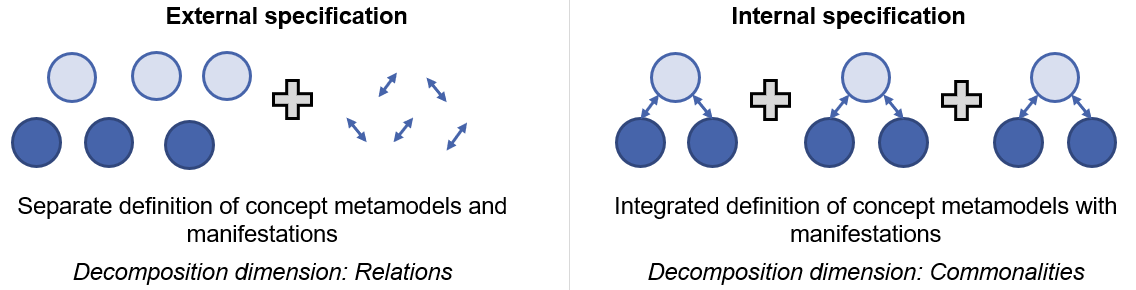
\includegraphics[width=\textwidth]{figures/quality/language/design_options.png}
    \caption[Design options for \commonalities specification]{Exemplification of alternatives to specify \commonalities by means of an integrated definition of \commonalities with their manifestation relations or the separate specification of complete \conceptmetamodels and manifestation relations.}
    \label{fig:language:design_options}
\end{figure}

\mnote{Decomposition dimensions}
We can distinguished two ways in which \conceptmetamodels and manifestation relations can be specified according to the \commonalities approach.
They depend on the dimension along which the specification is decomposed.
More precisely, the specification can either be decomposed along the \commonalities, such that each \commonalities together with all its manifestations is defined at one place, or it can be decomposed along the manifestation relations, such that all manifestation relations between a \conceptmetamodel and its manifestation are defined at one place.
We refer to these specifications as \emph{internal} and \emph{external} specification.
\begin{properdescription}
    \item[External concept definition:] \Conceptmetamodels are defined as ordinary metamodels and each manifestation relation is defined as an individual transformation, i.e., manifestation relations are defined externally to the \conceptmetamodels and their \commonalities.
    \item[Internal concept definition:] Each \commonality of each \conceptmetamodel is defined together with all its relations to its manifestations, i.e., manifestation relations are defined internally with the \commonalities they belong to.
\end{properdescription}
%We call the former way an \emph{internal} specification and the latter an \emph{external} specification, related to whether relations are defined internally with the \commonalities they belong to or as an external artifact.
We have proposed this distinction in previous work~\cite{klare2019models} and depict it in \autoref{fig:language:design_options}.

\mnote{External specification}
Without developing an additional language, the \commonalities approach can be realized by developing \conceptmetamodels as if they are ordinary metamodels with appropriate modeling tools.
The manifestation relations can then be defined with any existing transformation language that is able to generate incremental transformations, i.e., consistency preservation rules.
This conforms to an \emph{external} specification, in which \conceptmetamodels and manifestation relations are defined separately.
It decomposes the specification along the relations, thus there are many separate specification as there are \conceptmetamodels and manifestation relations to be defined, as depicted in the left of \autoref{fig:language:design_options}.
For example, for Java and \gls{UML} an object-oriented design \conceptmetamodel as well as two manifestation relations to each of the \concretemetamodels would be defined separately.

\mnote{Internal specification}
Developing a specific language allows to integrate the definition of \commonalities with their manifestation relations.
The relations to manifestation of a \commonality are then defined at one place with the declaration of the \commonality, improving locality of this related information.
This conforms to an \emph{internal} specification.
It decomposes the specification along the \commonalities, thus as many separate specification as \commonalities are defined exist, as depicted in the right of \autoref{fig:language:design_options}.
For example, for Java and \gls{UML} a class \commonality together with its manifestation as classes in both Java and \gls{UML} with the according relations of attribute values and references would be defined at one place.

\mnote{Tyranny of dominant decomposition}
Selecting one of these types of specification suffers from the \enquote{tyranny of the dominant decomposition}~\cite{tarr1999Tyranny-ICSE}.
This means, decomposition is only possible along one dimension of concerns, i.e., either the structural specification of \commonalities or the relational specification of manifestation relations, such that either one suffers from lacking separation of concerns in the other dimension.
Thus, while one approach improves locality when adding \commonalities, the other improves locality adding manifestation relations.

\mnote{External specification benefits}
External specifications benefit from the separation of each manifestation relation into its own specification.
This reduces dependencies between the manifestations and especially allows each developer who is responsible for a specific \concretemetamodel to define the relation to each related \conceptmetamodel as a whole instead of spreading his or her specification among all \commonalities specifications describing a concept represented in the \concretemetamodel.
In consequence, adding a new \concretemetamodel only requires the addition of manifestation relations to \conceptmetamodels and potentially updates to them.
This scenario is well supported by these kinds of specification, because locality of all information regarding a manifestation relation is high and the manifestation relations represent the largest part of the addition.
Additionally, this approach can be realized without developing a new language, as already discussed before.

\mnote{Internal specification benefits}
Internal specification require a dedicated language enabling the integrated specification of \commonalities and their manifestations.
This improves locality regarding the information about each \commonality, as each \commonality is represented along with all its manifestations.
In consequence, when initially developing \commonalities for a set of \concretemetamodels, it is easier to add each single \commonality, because all information about the \commonality and its relation to the manifestation can be defined at one place.
This can make it easier to understand the overall relation of that common concept among all \concretemetamodels.
In addition, it makes it more unlikely for a developer to miss the definition of one or more manifestations of a \commonality, as they are obviously missing in the specification of the \commonality, whereas in an external specification it is missing somewhere in the complete manifestation relation between the \conceptmetamodel and its manifestation.
Finally, the approach promises to be more concise, because the manifestation relations can be defined within the \commonality they belong to instead of referencing the \commonality within a transformation again.

\mnote{Proposal of internal specification language}
To benefit from locality regarding each \commonality and a more concise specification, we have decided to design a language that supports internal specifications.
Depending on the usage context and the more likely change scenarios, an external specification may, however, be more appropriate.
Then, modeling \concretemetamodels with existing modeling framework and the manifestation relations with existing transformation languages is sufficient.


\subsection{Artifacts and Process}

\mnote{Selected design options}
Regarding the design option in \autoref{chap:improvement:commonalities:operationalization} and \autoref{chap:language:design:internal_external}, we have made the following, already argued decisions.
First, we chose to operationalize a specification by treating \conceptmetamodels as ordinary metamodels, such that instances of them are created and kept consistent.
This option does especially not restrict expressiveness of the relations and the generation of additional models can be hidden from the user by appropriate tooling.
Second, we chose to provide a language that supports an internal specification of concepts to improve locality of the information regarding each \commonality.
We expect this specification to be more concise and to better support the initial specification process for \commonalities.

\begin{figure}
    \centering
    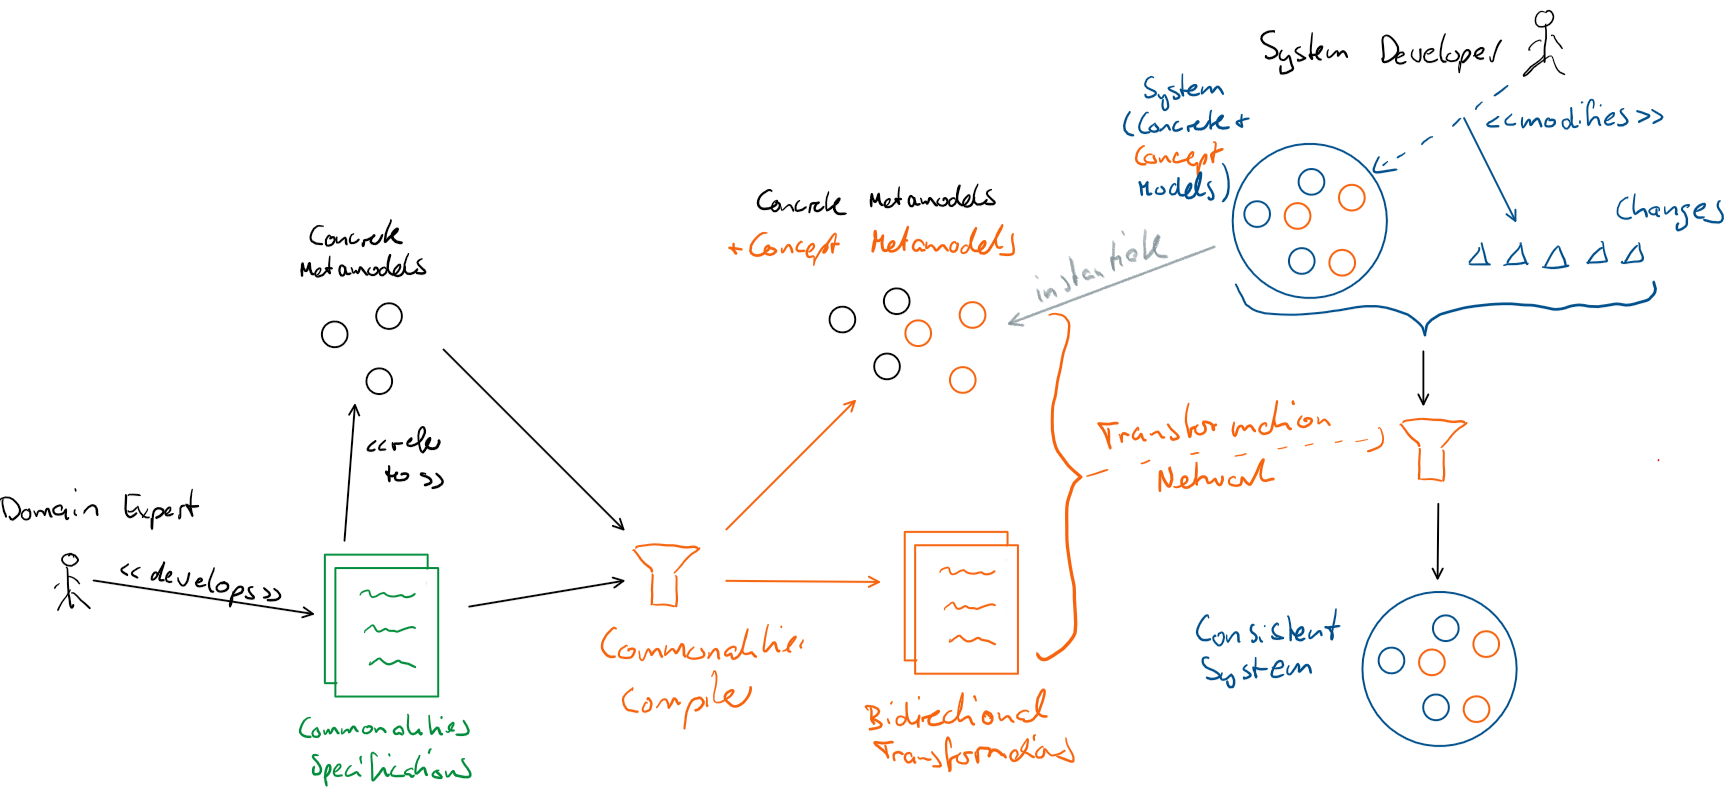
\includegraphics[width=\textwidth]{figures/quality/language/overall_process.png}
    \caption[Process and artifacts using a language for \commonalities]{The process for developing, compiling and executing specifications in a language for \commonalities. From \concretemetamodels and \commonalities specifications, additional \conceptmetamodels and transformations are generated, which are executed at runtime for preserving consistency of models.
    \Commonalities specifications by domain experts are marked green, the generated artifacts (\conceptmetamodels and transformations forming a network) are marked orange, and runtime artifacts including concrete systems and changes are marked blue.}
    \label{fig:language:process}
\end{figure}

\mnote{Specification and compilation}
The process of specifying, compiling and executing artifacts in such a language is depicted in \autoref{fig:language:process}.
It is a specialization of the general process already depicted in \autoref{fig:introduction:process_overview}.
A domain expert or transformation developer defines \commonalities specifications using the language, which refers to \concretemetamodels that are to be kept consistent by the transformations derived from that specification.
The compiler of the language takes the \concretemetamodels together with the specifications to generate a set of \conceptmetamodels in addition to the existing \concretemetamodels, as well as a set of bidirectional transformations, which implement consistency preservation for the manifestation relations between the \conceptmetamodels and \concretemetamodels.
These artifacts together form a transformation network, as introduced in \autoref{def:transformationnetwork}.

\mnote{Execution}
A system developer specifies a system by models that instantiate the \concretemetamodels of the \commonalities specification.
The complete system description consists of instances of these \concretemetamodels, but also, in the best case hidden from developer, of instances of the \conceptmetamodels for means of consistency preservation.
Whenever the system developer produces changes to the instances of the \concretemetamodels, the transformation network can be applied to the changes together with the models.
It then returns a new set of instances of the \concretemetamodel and \conceptmetamodels that are consistent again, according to the proposed correctness notion of transformation networks in \autoref{def:transformationnetworkcorrectness}.



\section{The \Commonalities Language}

\subsection{Elements Overview}
UML diagram or the like

\begin{figure}
    \centering
    \newcommand{\hdistance}{7.6em}
\newcommand{\classwidth}{5.5em}
\newcommand{\vdistance}{5em}

\begin{tikzpicture}[
    existing/.style={fill=lightgray!20}
]

\umlclassvarwidth[, existing]{metamodel}{}{Metamodel}{
name : String\\
}{\classwidth} 

\umlclassvarwidth[, existing, right=\hdistance of metamodel.north, anchor=north]{class}{}{Class}{
name : String\\
}{\classwidth}  

\umlclassvarwidth[, existing, right=\hdistance of class.north, anchor=north]{reference}{}{Reference}{
name : String\\
}{\classwidth}

\umlclassvarwidth[, existing, right=\hdistance of reference.north, anchor=north]{attribute}{}{Attribute}{
name : String\\
}{\classwidth}

\umlclassvarwidth[, below=\vdistance of metamodel.north, anchor=north]{concept}{}{Concept}{
}{\classwidth}  

\umlclassvarwidth[, right=\hdistance of concept.north, anchor=north]{commonality}{}{Commonality}{
root : Boolean\\
}{\classwidth}

\umlclassvarwidth[, below=\vdistance of commonality.north, anchor=north]{manifestation}{}{Manifestation}{
}{\classwidth} 

\umlclassvarwidth[, right=\hdistance of manifestation.north, anchor=north]{commonality_reference}{}{Commonality\\Reference}{
}{\classwidth}

\umlclassvarwidth[, right=\hdistance of commonality_reference.north, anchor=north]{commonality_attribute}{}{Commonality\\Attribute}{
}{\classwidth}


\umlclassvarwidth[, below left=\vdistance and \hdistance of manifestation.north, anchor=north]{manifestation_class}{}{Manifestation\\Class}{
alias : String\\
single : Boolean\\
}{\classwidth}

\umlclassvarwidth[, below=\vdistance of manifestation.north, anchor=north]{manifestation_condition}{}{Manifestation\\Condition}{
dir : Direction\\
}{\classwidth}

\umlclassvarwidth[, below=\vdistance of commonality_attribute.north, anchor=north]{attribute_relation}{}{Attribute\\Relation}{
dir : Direction\\
}{\classwidth} 

\umlclassvarwidth[, below=\vdistance of commonality_reference.north, anchor=north]{reference_relation}{}{Reference\\Relation}{
dir : Direction\\
}{\classwidth} 

\umlclassvarwidth[, below=\vdistance of manifestation_condition.north, anchor=north]{manifestation_operator}{}{Manifestation\\Operator}{
}{\classwidth}

\umlclassvarwidth[, below=\vdistance of attribute_relation.north, anchor=north]{attribute_operator}{}{Attribute\\Operator}{
}{\classwidth} 

\umlclassvarwidth[, below=\vdistance of reference_relation.north, anchor=north]{reference_operator}{}{Reference\\Operator}{
}{\classwidth} 

\umlclassvarwidth[, below=\vdistance of reference_operator.north, anchor=north]{operand}{}{\textit{Operand}}{
}{\classwidth}

\umlclassvarwidth[, below left=\vdistance and \hdistance of operand.north, anchor=north]{manifestation_operand}{}{\textit{Manifestation}\\\textit{Operand}}{
}{\classwidth}

\umlclassvarwidth[, below right=\vdistance and 0em of operand.north, anchor=north]{literal_operand}{}{Literal\\Operand}{
}{\classwidth}

\umlclassvarwidth[, right=\hdistance of literal_operand.center, anchor=center]{direction}{}{\umlenumlabel\\Direction}{
\itshape
Bidirectional\\
Checkonly\\
Enforce\\
}{\classwidth}

\umlclassvarwidth[, below left=\vdistance and \hdistance of manifestation_operand.north, anchor=north]{manifestation_class_operand}{}{Manifestation\\Class\\Operand}{
}{\classwidth}

\umlclassvarwidth[, below left=\vdistance and 0em of manifestation_operand.north, anchor=north]{manifestation_attribute_operand}{}{Manifestation\\Attribute\\Operand}{
}{\classwidth}

\umlclassvarwidth[, below right=\vdistance and \hdistance of manifestation_operand.north, anchor=north]{manifestation_reference_operand}{}{Manifestation\\Reference\\Operand}{
}{\classwidth}


% INHERITANCE
\umlsubclassof{concept}{--}{metamodel}
\umlsubclassof{commonality}{--}{class}
\umlsubclassof{commonality_attribute}{--}{attribute}
\umlsubclassof{commonality_reference}{--}{reference}

\umlsubclassof{manifestation_operand}{|- ([yshift=-1.5em]operand.south) --}{operand}
\draw (literal_operand) |- ([yshift=-1.5em]operand.south);

\umlsubclassof{manifestation_class_operand}{|- ($(manifestation_attribute_operand.north)!0.5!(manifestation_operand.south)$) --}{manifestation_operand}
\draw (manifestation_attribute_operand) -- ($(manifestation_attribute_operand.north)!0.5!(manifestation_operand.south)$);
\draw (manifestation_reference_operand) |- ($(manifestation_attribute_operand.north)!0.5!(manifestation_operand.south)$);

% REFERENCES
%\umlassociationfromto{(class) -- node[uml cardinality end, pos=1, above right] {1} (metamodel)}
\umlcomposition{(metamodel.east) -- node[uml cardinality end, pos=1, above left] {*} (class.west|-metamodel.west)}
\umlcomposition{(concept.east) -- node[uml cardinality end, pos=1, above left] {*} (commonality.west|-concept.west)}
\umlcomposition{(class.east) -- node[uml cardinality end, pos=1, above left] {*} (reference.west|-class.east)}
\umlcomposition{([xshift=1em]class.north) -- ++(0,1em) -| node[uml cardinality end, pos=1, above right] {*} (attribute.north)}

\umlcomposition{(commonality) -- node[uml cardinality end, pos=1, above right] {*} (manifestation)}
\umlcomposition{([xshift=-1em]commonality.south east) -- ++(0,-1em) -|node[uml cardinality end, pos=1, above right] {*} ([xshift=1em]commonality_reference.north west)}
\umlcomposition{([yshift=0.5em]commonality.east) -| node[uml cardinality end, pos=1, above left] {*} ([xshift=-1.5em]commonality_attribute.north)}

\umlassociationfromto{([xshift=-1em]commonality_reference.north) |- node[uml cardinality end, pos=1, above right] {1} node[uml role end, pos=1, below right] {type} ([yshift=-1em]commonality.east)}

\umlcomposition{([xshift=1em]manifestation.south west) -- ++(0,-1.5em) -| node[uml cardinality end, pos=1, above left] {1..*} ([xshift=-1em]manifestation_class.north east)}
\umlcomposition{(manifestation) -- node[uml cardinality end, pos=1, above left] {*} (manifestation_condition)}
\umlcomposition{(commonality_attribute) -- node[uml cardinality end, pos=1, above left] {*} (attribute_relation)}
\umlcomposition{(commonality_reference) -- node[uml cardinality end, pos=1, above left] {*} (reference_relation)}

\umlaggregation{(manifestation_condition) -- node[uml cardinality end, pos=1, above left] {*} (manifestation_operator)}
\umlaggregation{(attribute_relation) -- node[uml cardinality end, pos=1, above left] {*} (attribute_operator)}
\umlaggregation{(reference_relation) -- node[uml cardinality end, pos=1, above left] {*} (reference_operator)}

\umlaggregation{([xshift=1em]manifestation_class.north west) |- node[uml cardinality start, pos=0, above right] {*} ++(-1.5em,\vdistance) |- ([xshift=-1em,yshift=1em]class.north) -- node[uml cardinality end, pos=1, above left] {1} ([xshift=-1em]class.north)}

\umlcomposition{(attribute_relation.west) -- ++(-0.8em,0) |- node[uml cardinality end, pos=1, below right] {*} (operand.east)}
\umlcomposition{(reference_relation.west) -- ++(-0.8em,0) |- node[uml cardinality end, pos=1, above left] {*} ([yshift=0.8em]operand.west)}
\umlcomposition{([yshift=-0.5em]manifestation_condition.west) -- ++(-0.8em,0) |- node[uml cardinality end, pos=1, above left] {*} node[uml cardinality end, pos=1, below left] {rightOperand} ([yshift=-0.8em]operand.west)}
\umlcomposition{([yshift=0.5em]manifestation_condition.west) -- ++(-1.1em,0) |- node[uml cardinality end, pos=1, above left] {*} node[uml cardinality end, pos=1, below left] {leftOperand} ([yshift=0.8em]manifestation_operand.west)}

\umlassociationfromto{([yshift=-0.8em]manifestation_operand.west) -| node[uml cardinality end, pos=1, below right] {1} ([xshift=-1em]manifestation_class.south)}
\umlassociationfromto{(manifestation_attribute_operand.south) -- ++(0,-0.8em) -| ([xshift=0.8em, yshift=-1.2em]attribute.south east) -| node[uml cardinality end, pos=1, below right] {1} ([xshift=1.5em]attribute.south)}
\umlassociationfromto{(manifestation_reference_operand.east) -| ([xshift=0.4em, yshift=-2em]attribute.south east) -| node[uml cardinality end, pos=1, below right] {1} ([xshift=1.5em]reference.south)}

\end{tikzpicture}
    \caption[\commonalities language elements]{Class diagram with the essential elements of the \commonalities language and their relations. Elements that exist independent from the language are depicted in the top row.}
    \label{fig:language:elements}
\end{figure}

Additional consolidation of Relations (manifestation Condition, Reference/Attribute Relation), of Operator and of Named elements possible

\subsection{Concept Metamodels}

\subsection{Commonalities and Manifestations}

Participations and participation conditions
call them participations or manifestation?

\subsection{Properties and Operators}
Implemented operators:
* Attribute mappings operators: Mappings between attributes
* Attribute reference operators: Mappings between attributes that serve as references, e.g., subpackages in UML and concept metamodel as explicit references whereas encoded as namespace attributes in classes in Java -> namespace attribute of Java class is mapped to package structure in UML
* Condition operators

References realized by participations and commonalities referencing other commonalities

Reuse mechanisms, libraries of operators

Discuss that in fact this is comparable to declarative transformation languages, esp. Mappings, but also QVT-R, so no deeper discussion.



\subsection{Textual Syntax}

Grammar or maybe only examples, due to not focusing on concrete language and complexity of the actual language.


\section{Operationalization of Transformations}

\subsection{Compiling to \reactions}
Commonalities compile to \reactions, which are proven complete and correct~\cite{kramer2017a}.


\subsection{Matching Manifestations}

\subsection{Executing Operators}

Operators are executed as soon as one of the used values (parameters) is changed


\section{Expected Benefits}

Especially usability benefits, no conceptual benefits (in contrast to the concept as such)

\subsection{Improving Comprehensibility}

\begin{figure}
    \centering
    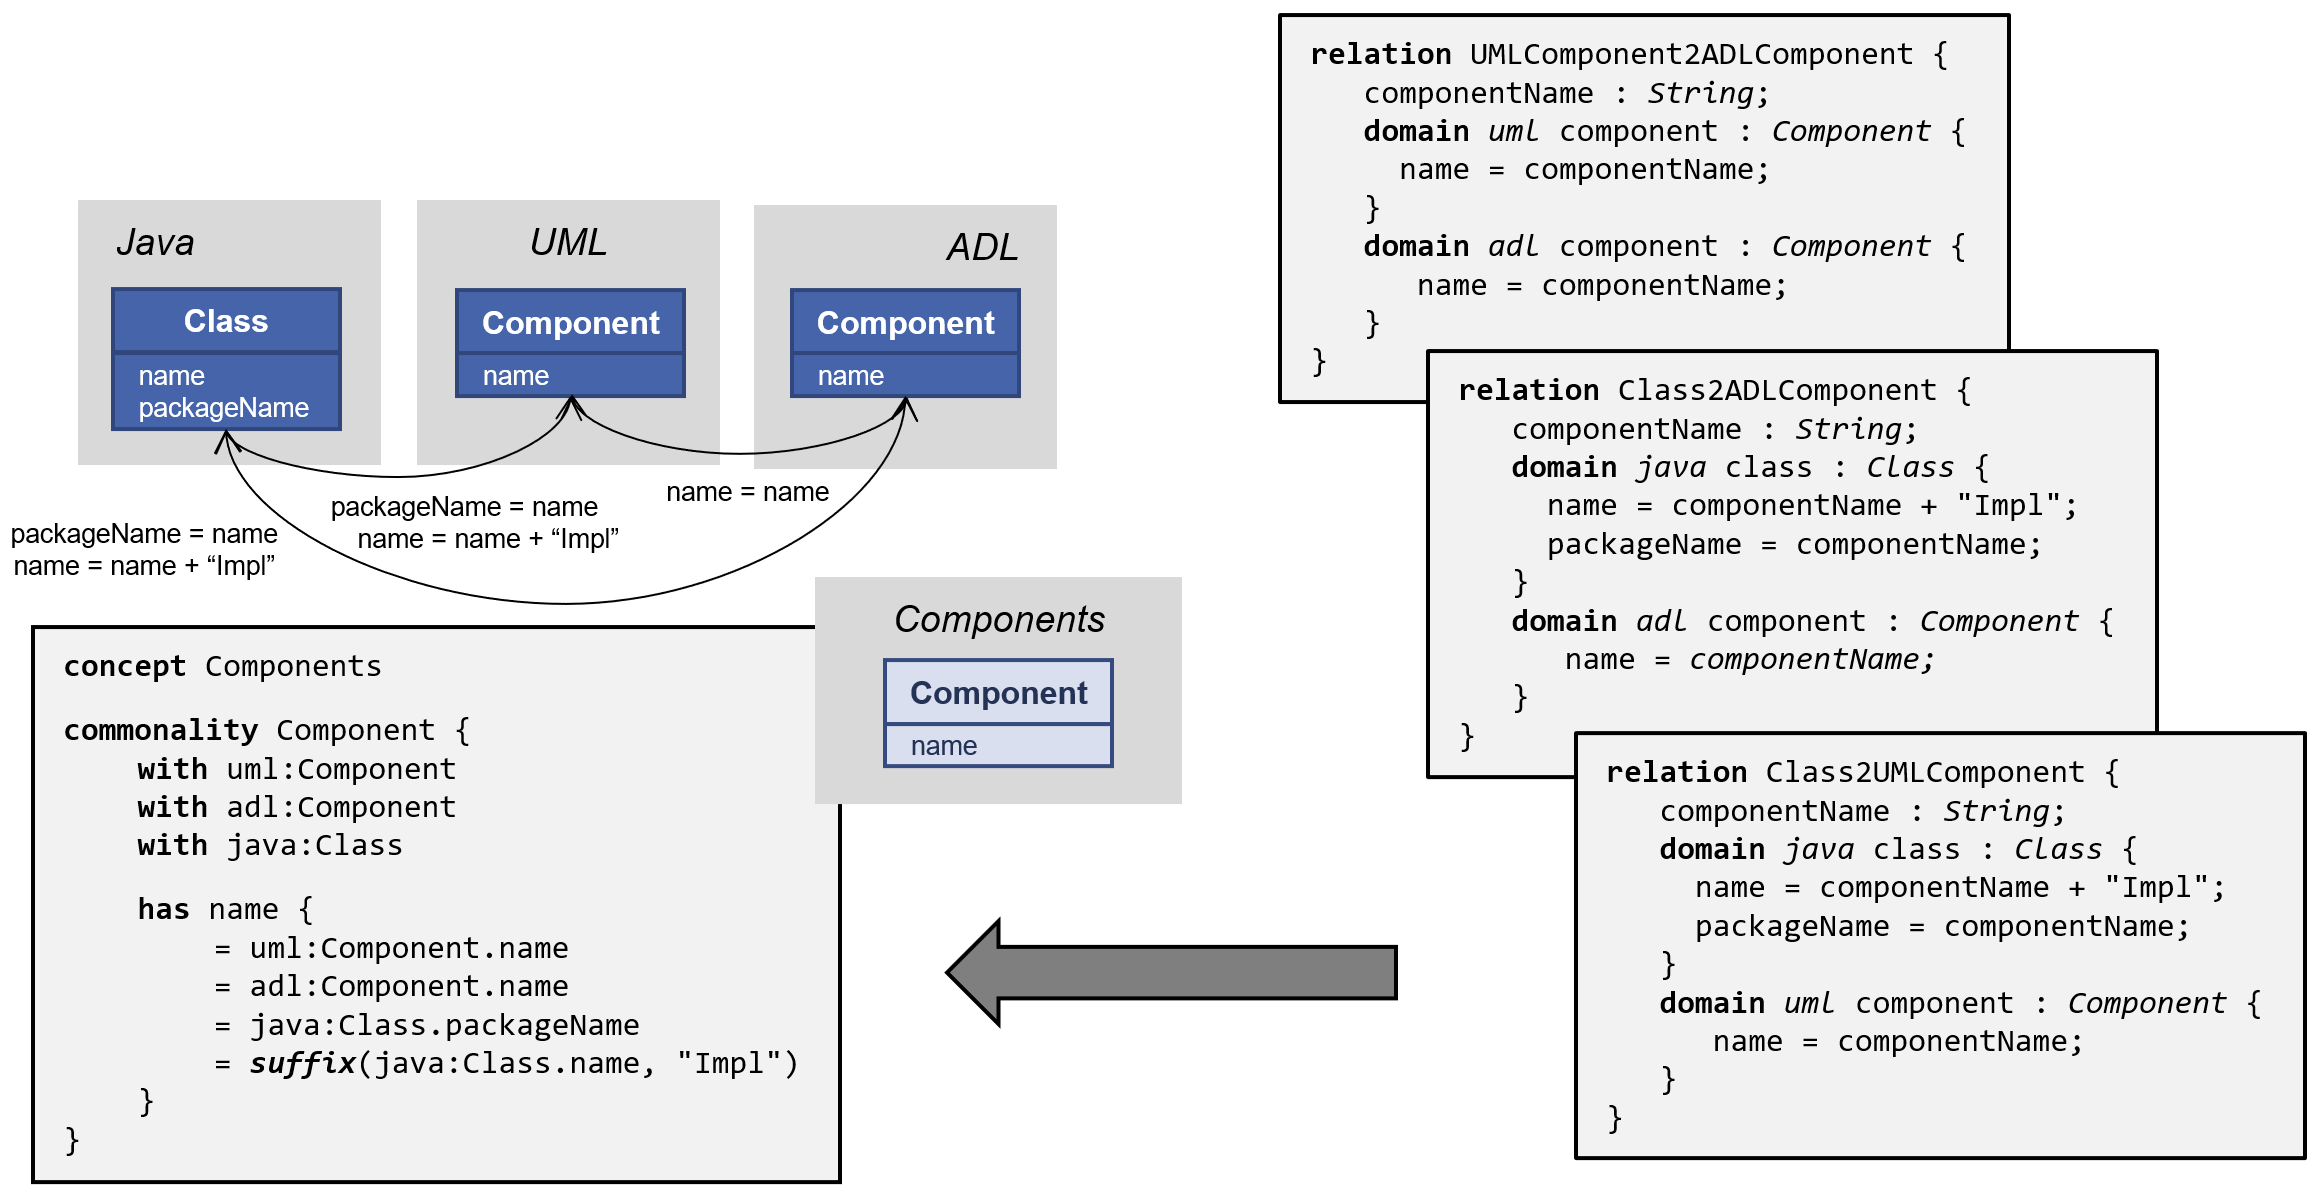
\includegraphics[width=\textwidth]{figures/quality/language/benefit_comprehensibility.png}
    \caption[Benefit of \commonalities regarding comprehensibility]{Example for consistency relations between classes and components expressed with \qvtr and the \commonalities approach.}
    \label{fig:language:benefit_comprehensibility}
\end{figure}

\subsection{Reducing Specification Effort}

Further benefit: Specification effort, adding concrete metamodel, adapting commonality, easier with internal specification


\section{Summary}

\begin{insight}{Language}

\end{insight}


\begin{copiedFrom}{VoSE}

% In this paper, we present the \emph{\commonalities approach}. %, which is based on the Bachelor's thesis of \textcite{gleitze2017a}.
% % Vorschlag:
% It defines \commonalities between metamodels explicitly and thereby allows to state clearly which common concepts they share.
% %, instead of encoding this information implicitly in a transformation.
% %The approach aims to explicitly define commonalities of metamodels for describing their consistency relations rather than implicitly encoding them in a transformation.
% From such a specification, transformations are derived that keep instances of those metamodels consistent.
% We discuss options how to derive such transformations, strategies to hierarchically compose \commonalities, as well as benefits and limitations of the approach.
% Additionally, we discuss design options for a language that supports the specification of \commonalities and present the \emph{\commonalities language}, which we have developed as a proof-of-concept.
% It is based on the Bachelor's thesis of \textcite{gleitze2017a}.

% Having introduced the concepts of the \commonalities approach, we now present the \commonalities language, as proposed by \textcite{gleitze2017a}.
% The language is a prototypical realization of the approach.
% We discuss design options for such a language and outline its syntax and its usage.
% This forms our contribution~\autoref{contrib:quality:language}.
% For a detailed discussion of the language capabilities, we refer to \cite{gleitze2017a}.
% In this paper, we focus on the presentation of fundamental concepts  and therefore only outline the language to give an impression of what our proof-of-concept evaluation is based on.


% \section*{Design Options}

% The development of a language for realizing the \commonalities approach provides at least two areas of design options.
% First, there are different possibilities to operationalize the approach, which covers decisions that are not visible to the user of the language.
% Second, different options regarding how to specify \conceptmetamodels and their relations to their manifestations exist, which are decisions that are visible to the user of the language.

% We already discussed in \autoref{chap:improvement:commonalities:operationalization} that there are two different options for operationalizing a specification of \commonalities: one that uses instances of the concept metamodels and defined transformations at runtime, and one that generates direct transformations between the \concretemetamodels from the specification.
% Since the way a specification is operationalized does not affect the user of the approach, it is up to the language and its designer to choose one of the options.
% We chose to build a language following the former approach, because it does not limit the possible relations that can be expressed.
% %We chose to build a language following the former approach, because it produces less initial effort to achieve a proof-of-concept that can be used to validate whether the approach is promising at all.

% Regarding the specification of \conceptmetamodels and the transformations, there are two options:
% \begin{description}[leftmargin=\parindent]
%     \item[External concept definition:] \Conceptmetamodels are defined as ordinary metamodels and the relations to their manifestation are defined in an individual transformation specification %, or even specifications in ordinary transformation languages, 
%     for each manifestation. %$\Rightarrow$ Benefit: Each Mapping independently specifiable
%     \item[Internal concept definition:] A specialized language allows to define the \conceptmetamodel and the \commonalities it consists of together with relations of all \commonalities to their manifestations. %$\Rightarrow$ Benefit: No elements accidentally missed \todoAll{Really or is there another benefit?}
% \end{description}

% A benefit of the first option is that the relation to each manifestation can be specified independently, which reduces dependencies between the different manifestations of one \conceptmetamodel.
% Additionally, it could be realized without developing a new language. The \conceptmetamodels can be described just like any other ordinary metamodel and one can use any existing transformation language, such as QVT, for the transformation definitions.
% The second option, in contrast, requires a dedicated language that enables an integrated specification of the \conceptmetamodel and its relations to manifestations.
% We chose to build a language following the second option because we expect its benefits to outweigh the mentioned disadvantages.
% First, it improves locality: all information about one \commonality is represented in one place.
% %instead of separating the \commonality definition from the transformation specifications.
% Because of that, we expect that it is easier for developers to understand the combined transformation logic concerning one \commonality.
% Additionally, the \conceptmetamodel can be easily extended with this solution whenever adding a manifestation requires defining a new \commonality.
% Finally, we expect that, compared to other options, grouping transformations by their \commonality reduces the possibility for developers to forget defining one or more relevant manifestations for a \commonality.
% %Finally, it is easier to ensure that for all \commonalities a relation to the manifestation is defined than in the first option, where \commonality specification and relation specification are separated.
% %Nevertheless, an obvious drawback of the second option in contrast to the first is that the mappings to the concrete metamodels cannot be specified independently but are tied to the Commonality definition.
% %Additionally, we expect that it makes it easier to understand the semantics of a \commonality and how it relates to its manifestations.}
% %and ensure that no elements are specified in the \conceptmetamodel that do have no manifestation in all relevant \concretemetamodels.


\section*{Language Description}

As introduced before, our realization of the \commonalities language
%for the previously explained \commonalities approach
provides an internal concept definition and uses the \conceptmetamodels as additional metamodels in the operationalization.
An example for the syntax of the \commonalities language is depicted in \autoref{lst:quality:commonalities_language_example}.

% \begin{figure}
%     \centering
%     \todo{Potentially extend running example so that references are covered. At least, we do not have the package in the example}
%     \includegraphics[width=\columnwidth]{figures/commonalities_language_example.PNG}
%     \caption{An example for defining the common concept of components}
%     \label{fig:commonalities_language_example}
% \end{figure}

\lstinputlisting[language=commonalities, float, belowskip=-0.8 \baselineskip,
    caption={[Exemplary commonality for components]An exemplary specification of the \texttt{Component} \commonality between \gls{PCM}, UML and the object-oriented design concept in the \commonalities language},
    captionpos=b,
    label=lst:quality:commonalities_language_example,
]{listings/quality/commonalities_language_example.lst}

The language allows to define \conceptmetamodels by declaring \commonalities, each representing one commonality between different manifestations, such as the \texttt{Component} \commonality in our example.
Relations between the \conceptmetamodels and their manifestations are supposed to be specified \emph{declaratively}.
%, which is realized as a \metaclass in the \conceptmetamodel.
For every \commonality, the \metaclasses in the manifestations that realize them are specified.
In the example, the \texttt{Component} in \gls{PCM} and the \texttt{Class} in the object-oriented design \conceptmetamodel are %defined as representations of
related to the \texttt{Component} \commonality.
In our language, a \commonality is realized by a \metaclass in the metamodel that is generated for a concept, so the \texttt{Component} \commonality is realized by a \texttt{Component} \metaclass.

Within a \commonality, attributes and references can be defined, similar to an ordinary \metaclass.
The relations of an attribute to the manifestation are declared directly at the attribute.
In the example, a \texttt{name} attribute is specified, which maps to the name of the component in \gls{PCM} and the name appended with an \enquote{Impl} suffix in Java.
The language %defined by \textcite{gleitze2017a} 
provides several operators for attribute relations, apart from equality relations.
The example depicts a prefix operator that allows to compose a String attribute.
Such operators can be defined independently and added to the language dynamically.
References can be defined comparably to attributes but can be enriched with a definition of containment relations.

% Introduce the idea of \enquote{Concepts} and \enquote{Commonalities}, explain how attributes and references are mapped.
% \todo{We have to align the definition of Concept, Commonality etc. in the paper with the implementation}

The actually conceptualized and implemented language by \textcite{gleitze2017a} is far more sophisticated than the simple overview we provide here. 
It supports different kinds of bidirectional operators for attribute mappings, containment specifications (so-called \emph{participations}), attribute checks as preconditions for \commonality instantiation, and more.

\end{copiedFrom} % VoSE
